\documentclass{beamer}
\usepackage{amsmath}
\usepackage{amssymb}
\usepackage{bm}
\usepackage{hyperref}
\usepackage{csquotes}
\usepackage{graphicx}

\DeclareSymbolFont{matha}{OML}{txmi}{m}{it}% txfonts
\DeclareMathSymbol{\varv}{\mathord}{matha}{118}
\usetheme{metropolis}

\graphicspath{ {pictures/Table_4_1.png}{pictures/Table_4_2.png}{pictures/Figure_3.png} }

\usefonttheme{serif} % default family is serif

\setbeamertemplate{section in toc}[sections numbered]
\setbeamertemplate{subsection in toc}[subsections numbered]

\title{Macroeconomics 3 Presentation}
\subtitle{Article review :  \\ Howell, Elliott, 
\textit{Damages Done: The Longitudinal Impacts of Natural Hazards on Wealth Inequality in the United States}, 2019}
\author{GUGELMO CAVALHEIRO DIAS Paulo \\ SHARMA Vivan}
\institute{Sciences Po}
\date{\today}

\begin{document}
\begin{frame}
    \titlepage
\end{frame}


\section{Introduction}

\begin{frame}{\secname}
    Study objects of the paper : 
    \begin{itemize}
        \item Contribution of Natural Hazards to Wealth Inequality
        \item Contribution of Insurance Policies to Wealth Inequality
    \end{itemize}
    Focus on the empirical facts : 
    \begin{itemize}
        \item The interaction between natural hazard and pre-existing social disparities
        \item The effect of private and public insurance
    \end{itemize}
\end{frame}

\begin{frame}
    \frametitle{Outline}
    \tableofcontents[hideallsubsections]
\end{frame}

\section{Study Design}

\subsection{Explaining Wealth with Socioeconomic Variables}
\begin{frame}{\subsecname}
    What is the effect of natural hazard on wealth inequalities ? 
    How does this effect vary in function of socioeconomic variables associated to an individual ? 

    \begin{equation*}
        f(\widehat{wealth}) = \widehat{\alpha} + \widehat{\beta} \cdot \log(\text{natural hazard damages}) + \widehat{\gamma} \cdot X
    \end{equation*}

    With $X$ socioeconomic variables (at the individual, local, and county levels) :

    Race, Foreign Born, Education, Married, Homeownership, Socioeconomic Status of the Neighborhood, etc...
    (discussed below)
\end{frame}

\subsection{Datasets}
\begin{frame}{\subsecname}
\begin{itemize}
    \item \textbf{Panel Study Income Dynamics (PSID)}
    \item \textbf{Spatial Hazard Events and Losses Database (SHELD)}
    \item \textbf{Census Data} 
    \item \textbf{Federal Emergency Management Agency (FEMA) Projects Summary (2016)}
\end{itemize}
\end{frame}

\begin{frame}{\subsecname}
    \textbf{Panel Study Income Dynamics (PSID)}
    \begin{itemize}
        \item From 1968 to now, with a modification of followed individuals in 1999.
        \item Used sample : from 1999 to 2013, with a two-years interview period. 
        \item Use of the restricted-access, geocoded version of the survey, with information on the neighborhood of the respondents.
    \end{itemize}
\end{frame}

\begin{frame}{\subsecname}
    \textbf{Spatial Hazard Events and Losses Database (SHELD)}
    \begin{itemize}
        \item Maintained by the Hazards and Vulnerability Research Institute (HVRI) from 1960 to now.
        \item They collect information on 18 types of natural hazards and their associated fatalities and property damages. 
    \end{itemize}
\end{frame}

\begin{frame}{\subsecname}
    \textbf{Census Data}
    \\ Three datasets, from two different census : 
    \begin{itemize}
        \item 2000 U.S. Decennial Census Long Form.
        \item 2006-2010 and 2011-2015 American Community Survey 5-year Summary Files.
    \end{itemize}
    Use : 
    \begin{itemize}
        \item Socioeconomic status of neighborhoods.
        \item Total population. 
        \item Urban / rural status. 
    \end{itemize}
\end{frame}

\begin{frame}{\subsecname}
    \textbf{Federal Emergency Management Agency (FEMA) Projects Summary (2016)}
    \begin{itemize}
        \item Immediate Needs Funding (INF).
        \item Individual and Household Program (IHP).
        \item Local housing vouchers, temporary units, financial grants, replacement of property, etc...
    \end{itemize}
\end{frame}

\section{Wealth Inequality : the general effects}

    \begin{frame}{\secname}
        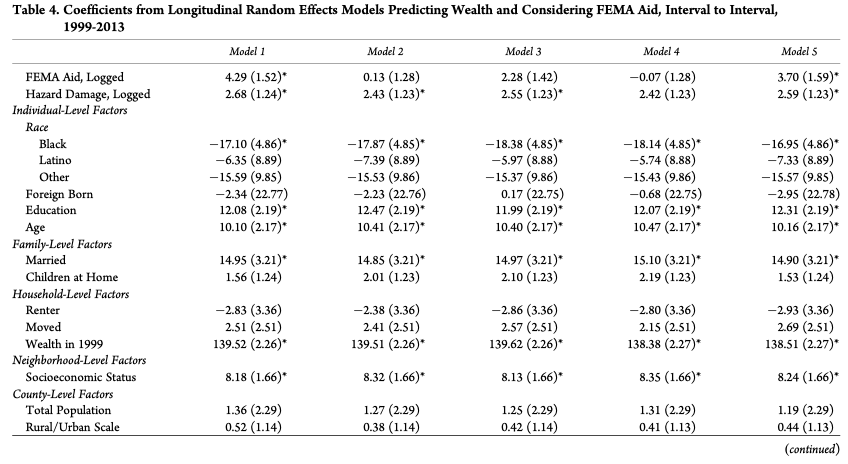
\includegraphics[totalheight=7cm,width=1\textwidth]{pictures/Table_4_1.png}
    \end{frame}

    \begin{frame}{\secname}
        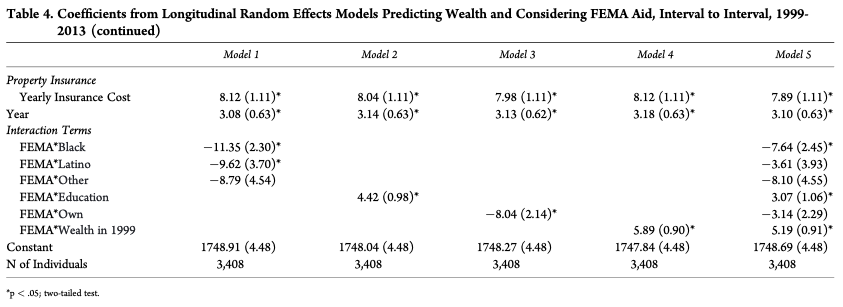
\includegraphics[width=1\textwidth]{pictures/Table_4_2.png}
    \end{frame}

    \begin{frame}{\secname}
        \textbf{Dollars :} For wealth, damages, and aid, everything is adjusted to 2012 dollars. All graphical illustrations are done with non-transformed dollars.
        \newline \hfill
        \newline \hfill
        \textbf{Wealth :} Definition of PSID, sum of saving accounts, checking accounts, real estate holdings, equity, vehicles,
        farms, businesses, stocks, annuities / IRAs, minus all reported debts. 
        Addition of a global minimum and use of square root.
        \newline \hfill
        \newline \hfill
        \textbf{Damages :} Due to right-skewed distribution, they use logarithm. Also, they standardize all values to 2012 dollars. 
        \newline \hfill
        \newline \hfill
        \textbf{Rural scale :} 1 corresponds to the most urban county, 9 to the most rural county. 
    \end{frame}


\section{Wealth Inequality : a concrete example}
    \begin{frame}{\secname}
        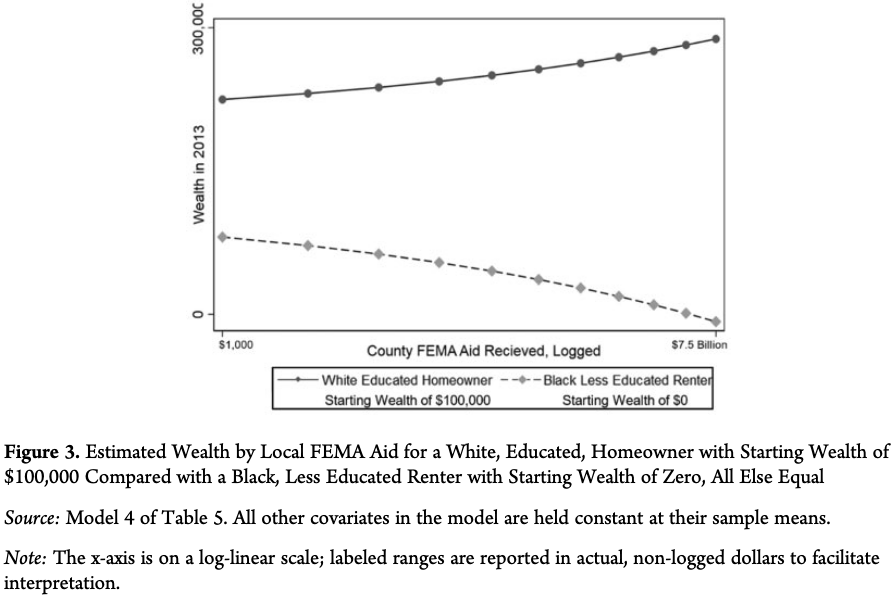
\includegraphics[totalheight=7cm,width=1\textwidth]{pictures/Figure_3.png}
    \end{frame}

\section{Conclusion}
    \begin{frame}{\secname}
        1. In a broader scale, natural hazards shocks provoke an increase in wealth disparities. 
        This paper points out \underline{the role of}
        \underline{natural hazards and insurance in the increase of the wealth gap}.

        2. Faced with environmental risks, agents are differently exposed not only due to budget constraints,
        but also due to \underline{lacking insurance schemes that would provide better} \underline{and more equitable
        coverage}.
        
        3. The authors call for further research on the precise mechanisms through which natural hazards affect wealth inequalities.
        They underly the need for a \underline{reform of} \underline{the current insurance system}, too much based on wealth and not enough on vulnerability.
    \end{frame}

\end{document}